\documentclass[12pt]{article}
%%%%%%%%%%%%%%%%
% Packages
%%%%%%%%%%%%%%%%

\usepackage[top=2cm,bottom=2cm,left=2cm,right= 2cm]{geometry}
\usepackage[parfill]{parskip}
\usepackage{graphicx, fontspec, xcolor,multicol, enumitem, setspace, amsmath, changepage}
\DeclareGraphicsRule{.tif}{png}{.png}{`convert #1 `dirname #1`/`basename #1 .tif`.png}

%%%%%%%%%%%%%%%%
% User defined colors
%%%%%%%%%%%%%%%%

% Pantone 2015 Fall colors
% http://iwork3.us/2015/02/18/pantone-2015-fall-fashion-report/
% update each semester or year

\xdefinecolor{custom_blue}{rgb}{0, 0.32, 0.48} % FROM SPRING 2016 COLOR PREVIEW
\xdefinecolor{custom_darkBlue}{rgb}{0.20, 0.20, 0.39} % Reflecting Pond  
\xdefinecolor{custom_orange}{rgb}{0.96, 0.57, 0.42} % Cadmium Orange
\xdefinecolor{custom_green}{rgb}{0, 0.47, 0.52} % Biscay Bay
\xdefinecolor{custom_red}{rgb}{0.58, 0.32, 0.32} % Marsala

\xdefinecolor{custom_lightGray}{rgb}{0.78, 0.80, 0.80} % Glacier Gray
\xdefinecolor{custom_darkGray}{rgb}{0.35, 0.39, 0.43} % Stormy Weather

%%%%%%%%%%%%%%%%
% Color text commands
%%%%%%%%%%%%%%%%

%orange
\newcommand{\orange}[1]{\textit{\textcolor{custom_orange}{#1}}}

% yellow
\newcommand{\yellow}[1]{\textit{\textcolor{yellow}{#1}}}

% blue
\newcommand{\blue}[1]{\textit{\textcolor{blue}{#1}}}

% green
\newcommand{\green}[1]{\textit{\textcolor{custom_green}{#1}}}

% red
\newcommand{\red}[1]{\textit{\textcolor{custom_red}{#1}}}

%%%%%%%%%%%%%%%%
% Coloring titles, links, etc.
%%%%%%%%%%%%%%%%

\usepackage{titlesec}
\titleformat{\section}
{\color{custom_blue}\normalfont\Large\bfseries}
{\color{custom_blue}\thesection}{1em}{}
\titleformat{\subsection}
{\color{custom_blue}\normalfont}
{\color{custom_blue}\thesubsection}{1em}{}

\newcommand{\ttl}[1]{ \textsc{{\LARGE \textbf{{\color{custom_blue} #1} } }}}

\newcommand{\tl}[1]{ \textsc{{\large \textbf{{\color{custom_blue} #1} } }}}

\usepackage[colorlinks=false,pdfborder={0 0 0},urlcolor= custom_orange,colorlinks=true,linkcolor= custom_orange, citecolor= custom_orange,backref=true]{hyperref}

%%%%%%%%%%%%%%%%
% Instructions box
%%%%%%%%%%%%%%%%

\newcommand{\inst}[1]{
\colorbox{custom_blue!20!white!50}{\parbox{\textwidth}{
	\vskip10pt
	\leftskip10pt \rightskip10pt
	#1
	\vskip10pt
}}
\vskip10pt
}

%%%%%%%%%%%
% App Ex number    %
%%%%%%%%%%%

% DON'T FORGET TO UPDATE

\newcommand{\appno}[1]
{4.1}

%%%%%%%%%%%%%%
% Turn on/off solutions       %
%%%%%%%%%%%%%%

% Off
\newcommand{\soln}[2]{$\:$\\ \vspace{#1}}{}

%%% On
%\newcommand{\soln}[2]{\textit{\textcolor{custom_red}{#2}}}{}

%%%%%%%%%%%%%%%%
% Document
%%%%%%%%%%%%%%%%

\begin{document}
\fontspec[Ligatures=TeX]{Helvetica Neue Light}

Dr. \c{C}etinkaya-Rundel \hfill Sta 101: Data Analysis and Statistical Inference \\
Duke University - Department of Statistical Science \hfill \\

\ttl{Application exercise \appno{}: \\
Zinc levels}

\inst{$\:$ \\
Team name: \rule{10cm}{0.5pt} \\
$\:$ \\
Lab section: $\qquad$ 8:30 $\qquad$ 10:05 $\qquad$ 11:45 $\qquad$ 1:25 $\qquad$ 3:05$\qquad$ 4:40 \\
$\:$ \\
Write your responses in the spaces provided below. WRITE LEGIBLY and SHOW ALL WORK! 
Only one submission per team is required. One team will be randomly selected and their 
responses will be discussed and graded. Concise and coherent are best!}

%%%%%%%%%%%%%%%%%%%%%%%%%%%%%%%%%%%%

\begin{enumerate}

\item Trace metals in drinking water affect the flavor and an unusually high concentration can pose a 
health hazard. Ten pairs of data were taken measuring zinc concentration in bottom water and surface 
water at 10 randomly sampled locations. The distributions are shown below. We want to evaluate 
whether the true average concentration in the bottom water \emph{exceeds} that of surface water? 
Note that water samples collected at the same location, on the surface and in the bottom, cannot be 
assumed to be independent of each other. The differences are calculated as $bottom - surface$.

\begin{center}
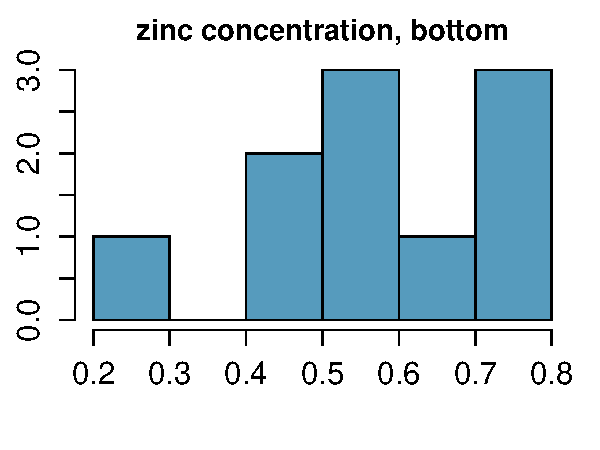
\includegraphics[width=0.3\textwidth]{figures/zinc/zinc_bottom_hist}
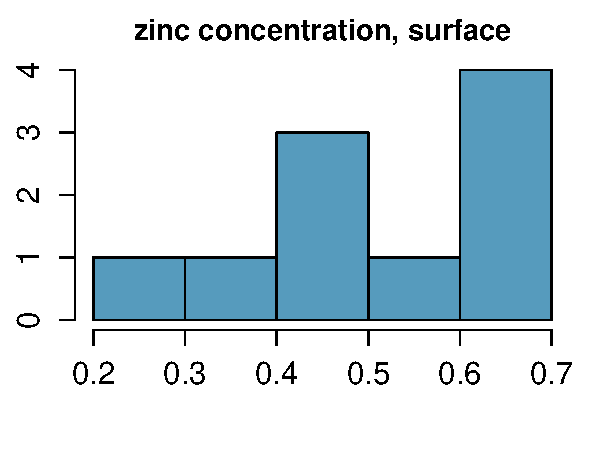
\includegraphics[width=0.3\textwidth]{figures/zinc/zinc_surface_hist}
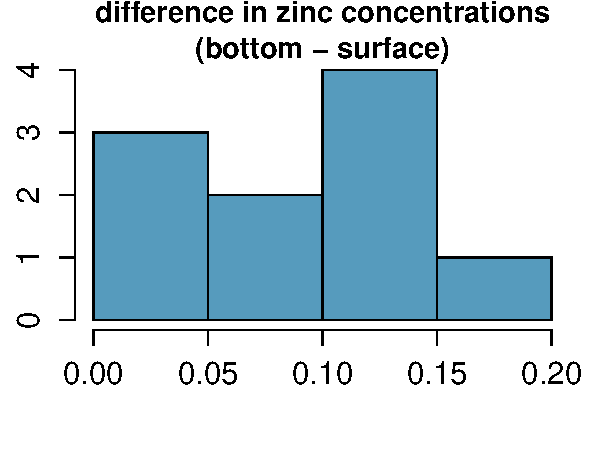
\includegraphics[width=0.3\textwidth]{figures/zinc/zinc_diff_hist}
{\small
\begin{tabular}{lccc}
\hline
			& $\bar{x}$ 	& $s$	& $n$ \\
\hline
bottom		& 0.5649		& 0.1468	& 10 \\
surface		& 0.4845		& 0.1312	& 10 \\
diff			& 0.0804		& 0.0523	& 10 \\
\hline
\end{tabular}
}
\end{center}

\begin{enumerate}

\item Define the parameter of interest and the point estimate, and state the value of the point estimate.

\soln{4cm}{Parameter of interest: Average difference between the zinc concentrations between bottom and surface water. \\
Sample statistic: Average difference between the the zinc concentrations between bottom and surface water in the observed data.}

\pagebreak

\item Conduct a hypothesis test answering the research question. Don't forget to check conditions first. 
Use $\alpha = 0.05$. Make sure to frame your conclusion in context of the data and the research question.

\soln{5cm}{
$H_0: \mu_{diff} = 0$ \\
$H_A: \mu_{diff} > 0$ \\
Conditions:
\begin{enumerate}
\item Independence: If the locations are sampled randomly one location can be assumed to be independent of another.
\item Skew: The distribution of differences is not extremely skewed.
\end{enumerate}
Hence we can assume that the sampling distribution of the average difference in zinc concentrations between bottom and 
surface water is nearly normal.
$T_{10 - 1} = \frac{0.0804 - 0}{\frac{0.0523}{\sqrt{10}}} = 4.86$ \\
p-value < 0.005 $\rightarrow$ Reject $H_0$, the data provide convincing evidence of a difference between in zinc 
concentrations between bottom and surface water.
}

\item Calculate a confidence interval for the parameter of interest at the confidence level equivalent 
to the previous hypothesis test. Make sure to interpret the interval in context of the research question.

\soln{6cm}{
CL: $1 - 0.05*2 = 0.90$
$0.0804 \pm 1.83 \frac{0.0523}{\sqrt{10}} = 0.0804 \pm 0.03 = (0.0504, 0.1103)$
We are 90\% confident that the zinc concentration in bottom water is 0.0504 to 0.1103 higher than surface water.
}

\end{enumerate}

%

\item Since 2005, the American Community Survey polls $\sim$3.5 million households yearly. The 
following summarizes distribution of salaries of males and females from a random sample of 
individuals who responded to the 2012 ACS:

\begin{center}
%
{\small
\begin{tabular}{lccc}
\hline
			& $\bar{x}$ 	& $s$	& $n$ \\
\hline
male			& 55,890		& 68,767.88	& 470 \\
female		& 29,240		& 32,025.98	& 373 \\
\hline
\end{tabular}
}
%
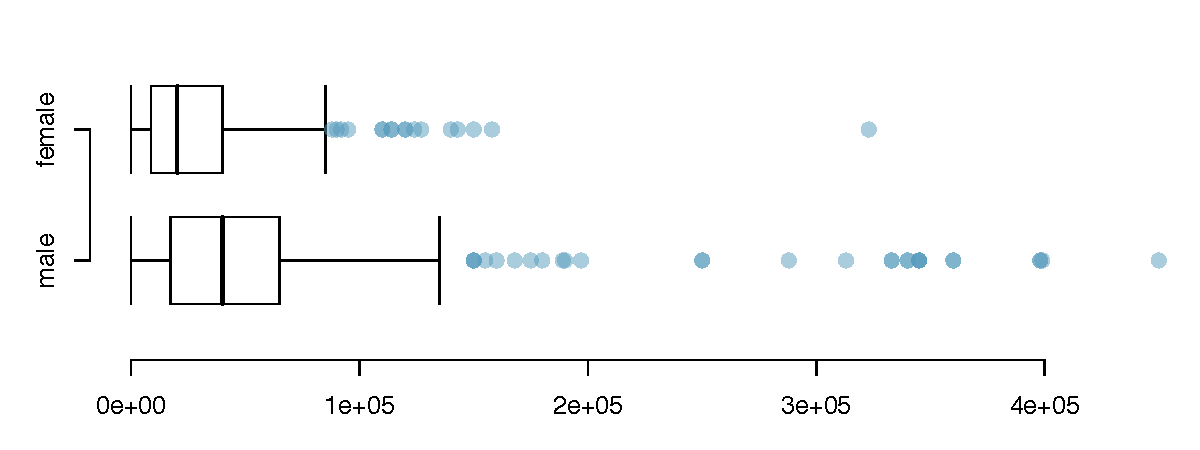
\includegraphics[width=0.8\textwidth]{figures/acs/sal_gen_box}
\end{center}
We want to evaluate whether salaries of men and women are different, on average.

\begin{enumerate}

\item Define the parameter of interest and the point estimate, and calculate the point estimate.

\soln{5cm}{Parameter: Difference in average salaries of all US males and females. \\
Statistic: Difference in average salaries of sampled males and females.
}

\item Conduct a hypothesis test answering the research question. Don't forget to check conditions first. Use 
$\alpha = 0.10$. Make sure to frame your conclusion in context of the data and the research question.

\soln{5cm}{
$H_0: \mu_{m} - \mu_{f} = 0$ \\
$H_A: \mu_{m} - \mu_{f} \ne 0$ \\
Conditions:
\begin{enumerate}
\item Independence: The individuals are randomly sampled and are less than 10\% of their respective populations.
\item Skew: The distributions are likely right skewed, but we have large sample sizes.
\end{enumerate}
Hence we can assume that the sampling distribution of the average difference in salaries of males and females
are independent of each other. \\
$T_{371} = \frac{(55,890 - 29,240) - 0}{\sqrt{\frac{68,767.88^2}{470} + \frac{32,025.98^2}{373}}} = \frac{26,650}{3,579.318} = 7.45$ \\
p-value < 0.01 $\rightarrow$ Reject $H_0$, the data provide convincing evidence of a difference in salaries of males and females.
}

\item Calculate a confidence interval for the parameter of interest at the confidence level equivalent to the 
previous hypothesis test. Make sure to interpret the interval in context of the research question.

\soln{5cm}{
$(55,890 - 29,240) \pm 1.97 \times 3,579.318 = (19,598.74, 33,701.26)$
We are 95\% confident that men on average make 19,598.74 to 33,701.2 more than women.
}

\end{enumerate}

\end{enumerate}

%%%%%%%%%%%%%%%%%%%%%%%%%%%%%%%%%%%%

\end{document}